% !TeX root = ../dissertation.tex

\newcommand{\codeat}[1]{\normalfont{\small Code at \texttt{#1}}}

\newcommand{\codesection}[2]{
      \section[#1]{#1\\\codeat{#2}}
}
\newcommand{\codesubsection}[2]{
      \subsection[#1]{#1\\\codeat{#2}}
}
\newcommand{\codesubsubsection}[2]{
      \subsubsection[#1]{#1\\\codeat{#2}}
}

%TC:macro \codeat 1
%TC:macro \codesection 2
%TC:macro \codesubsection 2
%TC:macro \codesubsubsection 2

\chapter{Implementation}

\begin{figure}[h]
      \centering
      \begin{tikzpicture}[auto,
                  node distance = 12mm,
                  start chain = going below,
                  box/.style = {draw, rounded corners, blur shadow, fill=white, on chain,
                              align=center, minimum height=8mm}
            ]

            \node[box] (ocaml) {OCaml Runtime};
            \node[box] (init) [right=of ocaml] {Initial Compiler};
            \node[box] (code) [below=of init] {Machine Code};
            \node[box] (opt) [right=of init] {Optimised Compiler};
            \node[box] (optcode) [below=of opt] {Optimised Machine Code};

            \begin{scope}[rounded corners, -latex]
                  \path (ocaml) edge (init) (init) edge (code) (code) edge (opt) (opt) edge
                  (optcode);
            \end{scope}
      \end{tikzpicture}

      \caption{Control flow through the compiler}
\end{figure}

I have developed two new JIT compilers from OCaml bytecode to x86\_64 assembly. The first compiler
completely replaces OCaml's bytecode interpreter and
is used for all programs and functions. The second is only used for functions that are called
multiple times at runtime.

\section{Overview}

OCaml bytecode is executed using a program called \texttt{ocamlrun}. Both new compilers are
implemented in a Rust static library that is linked with \texttt{ocamlrun}. \texttt{ocamlrun}
hooks into
this library when it loads bytecode and when it starts interpreting it.

If the JIT is enabled, either by setting an environment variable or compile-time setting, the
bytecode load hook will trigger the \textbf{initial compiler}.

The initial compiler parses the bytecode into a stream of instructions. For each bytecode
instruction it emits assembly with the same semantics to a buffer. After all code has been emitted
(including headers and footers with shared routines) relocations are performed and the buffer is
marked as executable.

When \texttt{ocamlrun} calls the hook to start interpretation, execution jumps to
this assembly code. The operations are performed in the same order as the interpreter - except
that every
instruction has been inlined.

When an OCaml closure is applied\footnote{All non-primitive function calls are translated to
      closure application.}, a closure execution count is incremented. Once this count passes a
configurable
threshold, the code instead branches to the \textbf{optimising compiler}.

The optimising compiler operates on the level of a single function. The code generated differs from
the unoptimised machine code in that there is no concept of the OCaml stack and accumulator
register; instead all values are stored in machine registers and the C stack. The function's code
pointer is updated and any
future calls (including the originally triggering call) will use the optimised implementation.

\section{Major milestones}

In accordance with the development methodology (see Section \ref{dev-methodology}) the focus
throughout all aspects of the project was on working code that could be tested. However, it is
worth
noting the order of major milestones, where some degree of full-system completeness was achieved.

\begin{enumerate}
      \item Execution of Hello World with the JIT.
      \item Passing the OCaml test suite and bootstrapping the compiler.
      \item Implementing the benchmark suite.
      \item (Extension) Implementing the optimising compiler.
\end{enumerate}

\section{Repository overview}

The project was developed using a `monorepo' where everything for the project was contained in one
Git repository. Some components are solely my work (marked \textbf{mine} below). Some components
are `vendored' (marked \textbf{vendor}) - where the source code is included to allow for small
patches to be made. For OCaml and the sandmark benchmark suites, the patches are significant enough
for me to consider it a fork containing both my work and the work of others (marked \textbf{fork}).

%TC:ignore
\dirtree{%
      .1 /.
      .2 benchmarks.
      .3 sandmark\DTcomment{\textbf{fork}: benchmark suite containing source \& tooling}.
      .3 analysis\DTcomment{\textbf{mine}: Jupyter notebooks analysing benchmark results}.
      .2 docs\DTcomment{\textbf{mine}: source of this document}.
      .2 scripts\DTcomment{\textbf{mine}: scripts to run tests and graph basic blocks}.
      .2 src.
      .3 rust.
      .4 ocaml-jit-shared\DTcomment{\textbf{mine}: shared code for the other two crates}.
      .4 ocaml-jit-staticlib\DTcomment{\textbf{mine}: crate that is linked with \texttt{ocamlrun}}.
      .4 ocaml-jit-tools\DTcomment{\textbf{mine}: binary crate with standalone tools}.
      .3 ocaml\DTcomment{\textbf{vendor}: contains OCaml compiler 4.11.1}.
      .4 runtime\DTcomment{\textbf{fork}: contains most large patches for the JIT}.
      .3 vendor\DTcomment{\textbf{vendor}: vendored rust dependencies with small patches}.
      .2 test-programs\DTcomment{\textbf{mine, vendor}: OCaml source for test programs}.
      .2 vendor/no-aslr\DTcomment{\textbf{vendor}: A simple wrapper to run a program without ASLR}.
}
%TC:endignore

\section{Initial compiler}

The initial compiler was developed before any work on the optimising compiler was performed. In the
process of implementing the initial compiler some modifications had to be made. These modifications
will be covered later in section \ref{dyn-recomp} and this section will mainly cover the initial
state.

\subsection{Overview}

The initial compiler consists of two major components - an instruction parser and an assembly
emitter. The instruction parser converts bytecode into Rust data types and the assembly emitter
translates the instructions into machine code.

\subsubsection{Mapping of the OCaml abstract machine}

Abstract-machine registers are mapped to x86\_64 registers. A pointer to the \texttt{Caml\_state}
struct containing other global interpreter state is also stored in a register called \texttt{r\_cs}
for access to its fields with small code size. The mapping used is shown in Table
\ref{table:regmap}.

\begin{table}[h]
      \centering
      \begin{tabular}{cc}\toprule
            OCaml register          & x86\_64 register \\
            \midrule                                   \\
            \texttt{r\_env}         & \texttt{r12}     \\
            \texttt{r\_accu}        & \texttt{r13}     \\
            \texttt{r\_extra\_args} & \texttt{r14}     \\
            \texttt{r\_sp}          & \texttt{r15}     \\
            \texttt{r\_cs}          & \texttt{rbx}     \\
            \bottomrule
      \end{tabular}

      \caption{Mapping of OCaml to x86\_64 registers.}
      \label{table:regmap}
\end{table}

Note that all x86\_64 registers mapped are callee-saved in the System V C calling convention. This
means that no work needs to be performed spilling and restoring them from the C stack to call
C/Rust
primitives (either as part of \texttt{CCall*} instructions or supporting primitives written for the
JIT).

\subsubsection{Mapping of the PC}

Bytecode pointers are mapped to native-code pointers and the interpreter's PC is replaced with the
system's instruction pointer. This change is responsible for nearly all of the performance
improvements of the JITed code. The benefits are

\begin{itemize}
      \item Memory accesses are reduced - rather than loading operands and opcodes, they are baked
            in to the machine code.
      \item The CPU can predict execution and fill its pipeline further than it can with the use of
            native code pointers.
      \item Branch prediction in hot paths becomes more effective as each branch can be predicted
            differently.
      \item The CPU can schedule out-of-order execution more effectively across different
            instructions.
\end{itemize}

However, this approach does lead to more contention on the instruction cache as instruction
implementation can no longer be shared, but this is offset by gains made elsewhere.

\codesubsection{Hooks from OCaml}{src/rust/ocaml-jit-staticlib/src/c\_entrypoints.rs}

The existing OCaml runtime was modified to hook into the JIT at three points:

\begin{enumerate}
      \item After a bytecode section is loaded.
      \item Before a bytecode section is released.
      \item When the interpreter is called.
\end{enumerate}

In most programs there is only one section loaded (two if callbacks from C to OCaml are
used). However, the interpreter is also used in the toplevel REPL where each section corresponds to
a line of code entered by the user toplevel.

Compilation happens after the first hook and an entry is written to a global table containing the
pointer to the buffer. The compiled code takes the form of a single large C taking no
arguments, meaning branching into the code consists only of calling a function pointer.

\subsection{Instruction parsing}

The first stage in the pipeline is to parse the bytes into a stream of elements of the
\texttt{Instruction} type.

\codesubsubsection{The \texttt{Instruction}
      type}{src/rust/ocaml-jit-shared/src/instructions/types.rs}
\label{instruction-type}

OCaml has 149 opcodes, each of which can take different numbers of operands. Arguments and operands
are all stored as \texttt{i32} values. Some opcodes are space-saving aliases for the composition of
multiple simpler instructions. To simplify implementation I expand these aliases at parse time, so
generating code only considers the simple primitives. There are about 60 such simplified
instructions.

Rust has support for algebraic sum types called enums. I use this to store the \texttt{Instruction}
type with one variant\footnote{Also known as type constructor.} per simple instruction.

Instructions such as integer comparisons and conditional branches have many variations varying only
in the conditional used. The variants are extracted into a type allowing for a single instruction
to
represent all conditional branches.

Some instructions, like branches, have label arguments referencing the location of another opcode
in
memory. The \texttt{Instruction} type is polymorphic over the type of the label to allow for
different label representations depending on use case.

\codesubsubsection{Parser}{src/rust/ocaml-jit-shared/src/instruction/parse.rs}

The parser is implemented using Rust iterators; the parser takes an iterator of \texttt{i32}s and
produces an iterator producing values of type \texttt{Result<Instruction, ParseError>}.

This use of iterators makes the instruction parser consistently performant for large programs -
consumers of the instruction stream take each instruction as they need rather than storing
a vector of all instructions in memory.

In OCaml bytecode, jumps are encoded as offsets relative to the current PC. To simplify later uses,
these are converted to absolute offsets relative to the start of the bytecode address.

As single OCaml instructions may parse to more than one \texttt{Instruction}, the type
contains a pseudo-instruction called \texttt{LabelDef}, which is emitted at
the start of every OCaml instruction. This also allows a map to be be built from labels to
locations in the translated code.

\codesubsection{Code generation}{src/rust/ocaml-jit-staticlib/src/compiler/emit\_code.rs}
\label{code-generation}

Code generation is the largest aspect of the compiler. It makes use of the \texttt{dynasm-rs}
library. This library manages emitting machine code and relocation information, relocating and
using \texttt{mmap} to mark the code as executable.

During this process \texttt{dynasm-rs} dynamic labels are used to set up relocations: these
labels are defined before every bytecode instruction and can be referenced by any other
instruction. \texttt{dynasm-rs} translates these at runtime into (machine PC)-relative jumps (as is
usual on x86\_64).

After all instructions are done, some shared code used by the instructions is emitted.
\texttt{dynasm-rs} then performs relocations and uses \texttt{mmap} to mark the region of code as
executable.

\subsubsection{Simple example}

The main code of the compiler itself is contained in a 2,000 line file
(\texttt{src/rust/ocaml-jit-staticlib/src/compiler/emit\_code.rs}). Most of this is taken up by a
Rust large pattern match for each of the bytecode instructions. As a very simple example of what
the code looks like, consider the implementation of the \texttt{ADDINT} opcode. It adds the value
at the top of the OCaml stack to the accumulator and stores the result in the accumulator. In the
original interpreter it is implemented:

\inputminted{c}{snippets/add.c}

Note that the OCaml integer format means a decrement is required to keep a 1 is the LSB. In the
compiler the relevant case is:

\inputminted{rust}{snippets/add.rs}

This has exactly the same semantics as the interpreter source. At compile time, the macro component
of \texttt{dynasm-rs} translates it to:

\inputminted{rust}{snippets/add_comp.rs}

In this way most translation from assembly to machine code is performed at compile time. The byte
string above contains the machine code for those instructions. This strategy is very performant.

\subsubsection{Branches}

As an example of the label and relocation support, consider the \texttt{BranchCmp(Comp, i32, L)}
instruction. It
compares the current value of the accumulator to the \texttt{i32} constant using the condition (of
type \texttt{enum Comp {Lt, Gt, ... }}). If the condition is true it branches to the label,
otherwise it passes to the next instruction.

This is implemented:

\inputminted{rust}{snippets/branchcmp.rs}

The macros translate it to:

\inputminted{rust}{snippets/branchcmp_comp.rs}

This shows the assembler work still needing to be done at compile time - relocations.

\subsubsection{Other cases}

All other cases follow this pattern. Some more involved instructions call into C primitives
I wrote, instead but most of them inline the operations directly in hand-written assembly. The main
exception is function calling --- this is covered in Section \ref{dyn-recomp}.

\subsection{Implementation strategy}

Implementation was incremental and highly test-driven. The initial focus was on building a system
supporting only the opcodes required to run a hello world program. I then slowly expanded the
complexity of programs, using them to drive the implementation of new instructions and fixing of
bugs.

The implementation was remarkably efficient, proceeding according to my most optimistic plan. This
is mainly due to the trace comparison tooling.

\subsubsection{Trace comparison} \label{trace-comparison}

There is no formal specification for the OCaml interpreter. The semantics of the interpreter are
what
\texttt{interp.c} and other files in the runtime say they are. Given this, I decided to build
tooling to test the behaviour of my JIT-compiled code directly against the behaviour of the
interpreter.

I added support for tracing after every instruction in both the existing interpreter and the
JIT-compiled code. The log entry contains the instruction executed, state of all of the OCaml
registers and the top five entries on the stack.

A wrapper program (in the \texttt{ocaml-jit-tools} crate) runs a specified program with tracing
enabled twice simultaneously - one run uses the JIT and the other the existing interpreter.  For
every trace entry printed it compares the two lines. If there is a difference between the lines it
shows a diff and then exits, as shown in Figure \ref{fig:trace-comparison}.

As many of the values are pointers there is a risk of non-determinism making this comparison fail.
I used a small open-source wrapper program called \texttt{no-aslr} to disable ASLR\footnote{GPLv2
      licensed, \url{https://github.com/kccqzy/no-aslr}.}. In order to ensure
that the Rust code doesn't cause them to become unaligned, I ran the compiler regardless of whether
JITed code was enabled when tracing was enabled. These two things together worked well enough that
all of the memory addresses were aligned and deterministic. This is unlikely to be true in general
for all OS kernels and malloc implementations, but worked on Linux with glibc.

The only expected difference comes from the use of the machine PC rather than the bytecode PC --
instruction pointers, like return addresses on the stack, could differ. This required a special
case during the check.

I wrote a script to run 11 test programs under trace comparison, failing if any of them failed.
Running this frequently allowed me to test for regressions when making changes.

\begin{figure}[h]
      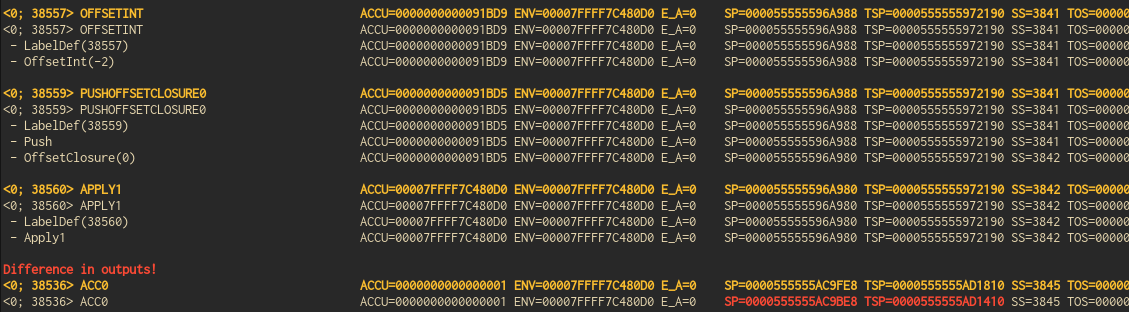
\includegraphics[width=\textwidth]{trace-comparison}
      \caption{Output on trace comparison failure.}
      \label{fig:trace-comparison}
\end{figure}

\subsubsection{Final stages}

Once I was happy that I had implemented every instruction, I started using
the OCaml compiler's internal test suite. I discovered some subtle bugs and used it to add new test
programs and fix them by trace comparison. One test heavily used callbacks from C to OCaml and I
discovered my initial implementation was too slow.

I eventually managed to get nearly all tests in the test suite working - the only failures were
testing the backtrace support and the debugger, which I had decided not to support in my proposal.
After this I successfully managed to bootstrap the compiler using the JIT which gave me a high
level of confidence in the accuracy of the JIT-compiled code.

\subsection{Omitted details}

Although the basic structure as described holds, some details are omitted but appear in
\texttt{emit\_code.rs}.

\begin{itemize}
      \item Callbacks from C to OCaml code require special handling.
      \item The compiler returns a pointer to the first instruction to support OCaml's
            metaprogramming \texttt{ocaml\_reify\_bytecode} function, used in the implementation of
            things like the
            toplevel \texttt{ocaml} program.
      \item Certain operations (like \texttt{ClosureRec(...)}) are involved enough that instead of
            inlining the definition in
            hand-written assembly, I push the registers to the C stack and call a C primitive to
            implement the
            operation (taking the registers as a struct).
      \item The compiler stores a persistent data structure of the sections to allow mapping
            bytecode addresses to machine-code addresses and allow for clean-up after a section is
            freed.
\end{itemize}

\section{Dynamic recompilation} \label{dyn-recomp}

The initial compiler, although a large piece software, does nothing that could not inherently be
done ahead-of-time with some more work on linking. The main benefit to operating as a JIT is it
allows for OCaml toplevel sessions to be JIT-compiled. Adding dynamic recompilation allows for the
system to discover hot paths in the code and optimise them more, which is something that requires
information about runtime behaviour. This is a popular technique for many existing optimising JITs,
like V8 for JavaScript.

The structure of the bytecode means it is natural to make the optimised compiler operate at the
granularity of a whole function, rather than a basic block or execution trace. Counting calls and
only branching to the optimising compiler above a certain threshold is a natural method for
determining hot functions and the method I decided to use.

However, allowing this required some changes to the initial compiler. In order to explain these
changes I first give an overview of how the OCaml interpreter deals with efficient
implementation of multiple arguments in the context of a functional language with partial
application.

\subsection{Existing OCaml calls} \label{exist-ocaml}

All functions in OCaml are implemented as closures - a heap-allocated tuple of a code pointer and a
list of data. Function calls are implemented as:

\begin{minted}{c}
check_stacks_and_signals(regs);
struct closure *c = (struct closure *) regs->env;
call_function(regs, f->code_ptr);
\end{minted}

Note the actual call logic is performed in hand-written assembly and these structs do not exist
anywhere
- this and subsequent examples are just pseudo-code. However, it is easier to understand the logic
at a higher level. \texttt{regs} is a pointer to a struct containing the OCaml registers - in the
actual assembly these are machine registers.

\subsubsection{Partial applications}

OCaml uses curried arguments allowing for the use of partial application:

\begin{minted}{ocaml}
# let add a b = a + b;;
val add : int -> int -> int = <fun>
# add 2 3;;
- : int = 5
# let add3 = add 3;;
val add3: int -> int = <fun>
# add3 5;;
- : int = 8
\end{minted}

In order to avoid making too many intermediate closures, OCaml has special support for this
extensively used pattern. All arguments are passed in order on the stack and the
\texttt{extra\_args}
register is used to mark how many arguments were used.

The number of arguments passed minus 1 is stored in the \texttt{extra\_args} register. The compiler
will insert a \texttt{GRAB(req\_extra\_args)} instruction at the start of any functions that take
more than one argument.  This instruction will cause an early return from the function if
\texttt{extra\_args} <
\texttt{passed\_extra\_args}. The return value will be a closure itself - this represents partial
application of curried functions. The data of this closure will be the arguments that were passed.
The code pointer of this returned closure points to a \texttt{RESTART} opcode immediately
preceding the grab, which moves the passed arguments off  the closure's data section onto the
stack, sliding them on top of any additional arguments passed.	Otherwise, it will subtract
\texttt{required\_extra\_args} from the \texttt{extra\_args} register
and continue executing.

This model is categorised as a push-enter model because it is the responsibility of the callee to
deal with arity mismatches.

\subsection{Function table}

In order to support dynamic recompilation, it is necessary to store the call count somewhere. A
naive method would be to store this in the closure as an extra data item, but this cannot support
optimising cases where the same code is used with different closure environments.

Instead, I modified the code pointer to point to a structure in memory. This structure is shared
between all closures using the same code. For now imagine it contains only one field: the code
pointer. Calls become:

\begin{minted}{c}
check_stacks_and_signals(regs);
struct closure *c = (struct closure *) regs->env;
struct function_metadata *f = c->code_ptr;
call_function(regs, f->code);
\end{minted}

\subsection{Moving the responsibility to the caller - eval/apply model}

I do not wish for optimised functions to do any of the work described in section \ref{exist-ocaml}.
As is described later, most of the speed increases of the optimised compiler comes from completely
eliminating use of the OCaml stack and the call method above makes heavy use of it.

Instead I shift the work to logically be performed by the caller. The way this is achieved is by
adding a
field storing \texttt{required\_extra\_args} to the function table and transforming the function
call to look something like this:

\begin{minted}{c}
check_stacks_and_signals(regs);
struct closure *c = (struct closure *) regs->env;
struct function_metadata *f = c->code_ptr;
if (regs->extra_args < f->required_extra_args) {
      // return partial application doing work of GRAB
} else {
      regs->extra_args -= f->required_extra_args;
      call_function(regs, f->code);
}
\end{minted}

I then modified the assembly translation of \texttt{GRAB} to be a no-op. Identical work is
performed but now it is the responsibility of the caller.

\subsection{Call counts and dynamic recompilation} \label{final-call-logic}

I added two new fields to the function-metadata struct: a reference to the original bytecode
location
of the function and a count/status variable.  The count/status is initialised to 0. Calls become:

\begin{minted}{c}
check_stacks_and_signals(regs);
struct closure *c = (struct closure *) regs->env;
struct function_metadata *f = c->code_ptr;
if (regs->extra_args < f->required_extra_args) {
      // return partial application doing work of GRAB
} else { 
      regs->extra_args -= f->required_extra_args;
      if (f->count_status == -1) {
            // Call the optimised function
            call_opt(regs, f->code);
      } else if (f->count_status == THRESHOLD_CALLS) {
            // Run the optimising compiler then call the optimised function
            f->code = optimising_compiler(f->original_bytecode_location);
            f->count_status = -1;
            call_opt(regs, f->code);
      } else {
            // Increment count and call the unoptimised function 
            f->count_status++;
            call_function(regs, f->code);
      }
}
\end{minted}

\subsection{Actual implementation}

Even though most of the above snippets are pseudo-code, the function-metadata struct as listed with
its four fields (code pointer, original bytecode location, required extra args, count/status)
exists in the compilation. Before implementing the optimising compiler, the initial compiler was
modified to generate, store and use it.

In order to generate this table, I added another pass to the initial compiler that discovers the
bytecode locations of all closures. This is performed by iterating through all functions. When a
\texttt{Closure(bytecode\_location, num\_vars)} bytecode operation is found (which creates a
closure) the code pointer is inspected. By inspecting the first instruction found at the bytecode
location, it is possible to find the value of the \texttt{required\_extra\_args} field.

After all the code is emitted, the function table is emitted. \texttt{dynasm-rs}'s relocations are
used to load the initial code pointers into the function table and link to the struct in the
closure table when compiling \texttt{Closure(...)} operations.

The net result of these changes is an extra pointer lookup being performed every time a function is
called. However this is necessary to allow dynamic replacement of functions with optimised
versions.

\section{Optimising compiler} \label{opt-comp}

The previous section laid out a way to determine hot closures and dynamically call into an
optimising compiler. This section describes the implementation of this optimising compiler and how
calls are done.

The time left for the project meant building a complete x86\_64 compiler backend (with register
allocation,
instruction scheduling, etc.) from scratch was infeasible. The usual toolkit used to avoid
replicating this work is LLVM \cite{llvm}. Although more typically known for its use in
ahead-of-time (AOT) compilation, there is some support for use in JITs. However, its large size and
complexity and AOT focus made it difficult to integrate.

\subsubsection{Cranelift}

Instead I used the cranelift library. Like LLVM it is a retargetable code generator with an IR.
However, it has a number of different design decisions that made it much better suited for my
planned uses:

\begin{itemize}
      \item It is written in Rust so the API follows Rust idioms.
      \item It is designed primarily for JITs and focuses heavily on compilation performance.
      \item Although the support for garbage collection is not extensible, it fits well with the
            OCaml garbage collector.
      \item When I encountered any bugs or missing features I could easily submit and get merged
            patches to the project --- I did this twice.
\end{itemize}

It didn't have all features I wanted but it is a good fit for my needs and was in a large part
responsible for my being able to complete this ambitious extension.

\subsection{Overview}

At a high level the optimised compiler is a function from function bytecode to optimised code
performing the same operations.  The compiler consists of three major components in a pipeline.

\begin{enumerate}
      \item Basic block conversion and stack-start analysis (section \ref{opt-bb}).
      \item IR generation from the basic blocks using the analysis (section \ref{opt-irgen}).
      \item Compilation of IR to x86\_64 assembly (performed by cranelift).
\end{enumerate}

\subsection{Optimisations performed}

The largest change from the initial compiler to the optimised compiler is that it no longer
generates
code that uses the OCaml stack and accumulator registers. This is achieved by replacing these uses
of the OCaml stack with machine registers that spill to the C stack when needed.

Arguments are passed to a function according to the System V C calling convention - the first
argument is always the closure environment, \texttt{env}, and the remaining arguments are passed
in registers (further details are given later in Section \ref{calling-conventions}). The work done
of Section \ref{dyn-recomp} means the function will only be called with the complete number of
arguments it is expecting.

The method used to remove the use of the stack is to convert the OCaml bytecode into an SSA form
by keeping track of the contents of a virtual stack and accumulator as the closure is translated.
Consider the simple OCaml function:

%TC:ignore
\mint{ocaml}|let add a b = a + b|
%TC:endignore

The OCaml compiler produces this sequence of bytecode instructions:

%TC:ignore
\begin{verbatim}
Grab(1)          # Ensure 2 arguments passed
Acc(1)           # Load 2nd element from top of stack (arg a) to acc
Push             # Push acc onto top of stack
Acc(1)           # Load new 2nd element from top of stack (arg b) to acc
ArithInt(Add)    # Add the top of stack to the acc and pop it
Return(2)        # Pop 2 items, then return acc (now a + b)
\end{verbatim}
%TC:endignore

\begin{table}[h]
      \centering
      \begin{tabular}{ccc}\toprule
            Initial state                   & Operation              & Final state
            \\
            \midrule
            \\
            \texttt{acc=?, stack=[b, a]}    & \texttt{Acc(1)}        & \texttt{acc=a, stack=[b, a]}
            \\
            \texttt{acc=a, stack=[b, a]}    & \texttt{Push}          & \texttt{acc=a, stack=[a, b,
                              a]}
            \\
            \texttt{acc=a, stack=[a, b, a]} & \texttt{Acc(1)}        & \texttt{acc=b, stack=[a, b,
                              a]}
            \\
            \texttt{acc=b, stack=[a, b, a]} & \texttt{ArithInt(Add)} & \texttt{acc=a+b, stack=[b,
                              a]}
            \\
            \texttt{acc=a+b, stack=[b, a]}  & \texttt{Return(2)}     & \texttt{acc=a+b, stack=[]}
            \\
            \bottomrule
      \end{tabular}

      \caption{Translation of add.}
      \label{table:stacktrans}
\end{table}

Instead of translating all of these inefficient stack manipulations as the initial compiler does,
the optimised compiler keeps track of the stack as it compiles. For an example of this, see Table
\ref{table:stacktrans}.

\codesubsection{Conversion to basic blocks}{src/rust/ocaml-jit-shared/src/basic\_blocks/}
\label{opt-bb}

The typical data structure used in optimising compilers is the basic block. Cranelift is no
exception and the IR for a function consists of basic blocks containing instructions in SSA form
with block parameters.

However, the only information we have from the bytecode is a sequence of instructions with jumps.
In order to move away from a heavy connection with the instructions the first step is to group them
into basic blocks. These bytecode-instruction basic blocks are then translated into cranelift basic
blocks.

\codesubsubsection{Types}{basic\_blocks/types.rs}

A \texttt{BasicClosure} consists of a vector of \texttt{BasicBlock} along with
some other data. A basic block has a vector of \texttt{BasicBlockInstruction} and a single
\texttt{BasicBlockExit}.

Some \texttt{Instruction}s map to a \texttt{BasicBlockInstruction} and others map to a
\texttt{BasicBlockExit}. For example, \texttt{Instruction::Push} becomes
\texttt{BasicBlockInstruction::Push} but \texttt{Instruction::BranchIf(label)} becomes
\texttt{BasicBlockExit::BranchIf \{ then\_block, else\_block \}}. This enforces at the type level
the basic invariant of basic blocks - one entry, one exit.

\subsubsection{Stack starts}

In addition to performing the conversion to basic blocks, the algorithm also keeps track of a
concept I call the \emph{stack start} of a basic block. Inspecting the bytecode compiler's source
and validating with many programs finds an important invariant:

\begin{framed}
      \noindent
      For all paths leading from the entry block of a function to an instruction, the absolute
      stack size
      relative to the start of the function's stack frame is the same.
\end{framed}

During the conversion the size of the stack on entry to each block stored. This is the \emph{stack
      start} of the block.

\codesubsubsection{Algorithm}{basic\_blocks/conversion.rs}

The algorithm consists of two iterations of depth-first search (DFS). The first finds all bytecode
offsets that form the start of blocks. The second visits all these blocks working out stack sizes.

In order to describe this algorithm without too many OCaml-specific confusing details I will
demonstrate it with
a simplified model:

The first DFS pass is only necessary to deal with loop back edges. For simplicity let's assume this
doesn't happen.

Let \(I\) be the set of all instructions. The program \(P\) is a list of instructions and can be
indexed. \(P\) can be thought of as a function \(\mathbb{N} \to I\).
For simplicity, assume indices are consecutive\footnote{They're not, but it's fairly simple to
      handle.}.

Each instruction has four properties. With $\mathbb{B} = \{ \textbf{true}, \textbf{false} \}$,
define:

\begin{itemize}
      \item \(\delta(i) : I \to \mathbb{N} \) is the change to the stack pointer after executing
            the
            instruction. For
            example, \texttt{Push}, which pushes the acc to the stack has, \(\delta(\texttt{Push})
            =
            +1\).
      \item \(\dfsexit(i) : I \to \mathbb{B} \) is \textbf{true} iff the instruction causes
            the block to end
            (jumps, returns).
      \item \(\dfsfallthrough(i) : I \to \mathbb{B} \) is \textbf{true} iff \(\dfsexit(i)\)
            and it can end up
            jumping to the following instruction. \texttt{BranchIf(branch\_loc)} is fallthrough but
            \texttt{Branch(branch\_loc)} is not.
      \item \(\dfslabels(i) : I \to \mathcal{P}(\mathbb{N}) \) is the set of all labels the
            instruction could end up jumping to
            (not
            including falling through). For example, \(\dfslabels(\texttt{BranchIf(branch\_loc)}) =
            \{\text{branch\_loc}\}\). It is only relevant if \(\dfsexit(i)\).
\end{itemize}

Under this model, the algorithm to find all the blocks and their starts is shown in algorithm
\ref{alg-dfs}.

\begin{algorithm}[t]
      \caption{DFS to find basic blocks and their starts}\label{alg-dfs}
      \begin{algorithmic}[1]
            \Function{FindBlocks}{$P, arity$}
            \State $seen \gets \emptyset$
            \State $starts \gets \{\}$
            \Function{VisitBlock}{$initial\_index, initial\_stack\_size$}
            \If{$initial\_index \in seen$}
            \Assert{$starts[initial\_index] = initial\_stack\_size$}
            \State \textbf{return}
            \EndIf
            \State $starts[initial\_index] \gets initial\_stack\_size$
            \State $i \gets initial\_index$
            \State $s \gets initial\_stack\_size$
            \Repeat
            \State $x \gets P[i]$
            \State $s \gets s + \delta(x)$
            \If{$\dfsexit(x)$}
            \For{$j \in \dfslabels(i)$}
            \State \Call{VisitBlock}{j, s}
            \EndFor
            \If{$\dfsfallthrough(x)$}
            \State \Call{VisitBlock}{i + 1, s}
            \EndIf
            \State \textbf{return}
            \EndIf
            \State $i \gets i + 1$
            \Until{forever}
            \EndFunction
            \State \Call{VisitBlock}{0, arity}
            \State \textbf{return} $starts$
            \EndFunction
      \end{algorithmic}
\end{algorithm}

\subsubsection{Additional operations performed during the search} \label{addop}

The algorithm, as presented in Algorithm \ref{alg-dfs}, shows only the basic logic of the search
and
storing of the stack starts for each block. The actual search also performs more work:

\begin{itemize}
      \item When a block is visited, a vector is created to hold the parsed instructions.
      \item Blocks are numbered in reverse post-order (the natural order for basic blocks where,
            with the exception of loop back edges, blocks are visited in a way consistent with
            execution order).
      \item Every time an instruction is visited, any labels referencing other blocks are replaced
            with the block ids and a copy is added to the vector.
      \item At exit, all of the block metadata is stored in a \texttt{BasicBlock} struct and placed
            in a table of blocks referenced by the block number.
      \item The maximum stack size at any point in the function is computed. It is used later in
            the IR generation phase.
\end{itemize}

\subsubsection{Example}

There isn't space to fit it in the main body of the text but Appendix \ref{appendix-example} shows
an example of the output of the basic block conversion for a larger function with if statements.

\subsection{Calling conventions} \label{calling-conventions}

In the initial interpreter, all calling is performed using the OCaml interpreter's existing model.
This
passes all arguments on the OCaml stack and has the caller deal with partial application and tail
calls.

We would like to avoid the stack in hot paths, so instead use a model where arguments are passed
according to the
System V calling convention. This is enabled by the changes made in Section \ref{final-call-logic}.

Values stored in the closure's environment need to be accessible to the function, so the first
argument is always a reference to the closure's environment. The remaining arguments correspond to
the function's arguments when fully applied with the arguments it expects.

The function returns two values: the return value of the function and another value which
corresponds to an \texttt{extra\_args} offset used for doing tail calls.\footnote{
      The details of this are beyond the scope of this dissertation --- it suffices to note this
      allows for tail calls even though cranelift doesn't support them.}

For example,

%TC:ignore
\mint{ocaml}|let add a b = a + b|
%TC:endignore

is translated to a function with signature

\begin{verbatim}
(env: i64, a : i64, b : i64) -> (i64, i64)
\end{verbatim}

The compiler can only process functions of up to five arguments, which corresponds to the maximum
number of arguments that can be passed in registers in the System V calling convention. This
simplifies the interface code and in practice nearly every function in the standard library can
work in this way.

\begin{itemize}
      \item Calls from from optimised code to optimised code can be implemented with simple C
            function calls
      \item Calls from the stack-using output of the initial compiler require the caller to read
            the arguments
            from the stack and call the function with this convention
      \item Calls from optimised code to unoptimised
            code require writing the arguments back to the OCaml stack
\end{itemize}

All of these cases are implemented in hand-written assembly, optimising for the first case
(optimised to optimised). This allows for the hot path sequence of calls to be without any need to
store arguments in memory.

\subsection{IR generation} \label{opt-irgen}

Cranelift, much like LLVM, uses an IR with a binary, in-memory and textual representation. IR is
stored in SSA form and each value has an associated type --- such as \texttt{I64} or \texttt{F32}.

IR generation starts by initialising the function header. Then every basic block is considered in
turn, emitting cranelift IR.

Although SSA form is very useful, it can be somewhat difficult to translate from higher level forms
where the same variable can hold multiple values. Cranelift provides some assistance with this
during the process of building the IR. This is similar to LLVM's \texttt{mem2reg} pass but more
direct, operating at the same time as IR is being built rather than as a separate optimisation
pass.

This functionality is the key method for removing use of the OCaml stack and accumulator. Cranelift
\texttt{Variable}s are defined to correspond to each stack location used in the function and the
accumulator.
Each variable needs a unique integer id. This allows cranelift to perform dataflow analysis to
track the loads and stores to the variable replacing them with SSA values.

\begin{minted}{rust}
let acc_var = Variable::new(0);
builder.declare_var(acc_var, types::R64);
let stack_vars: Vec<_> = (0..max_stack_size).map(|i| {
    let v = Variable::new(i + 1));
    builder.declare_var(acc, types::R64);
    v
}).collect();
\end{minted}

When emitting IR, cranelift provides functions to get a reference to the current value of a
variable
or set a new value.  The IR builder will track this against the control flow graph doing things
like automatically inserting block parameters (see Section \ref{ssa}).

For example, \texttt{PUSH} (push current accumulator to stack) is handled in this way:

\begin{minted}{rust}
let current_acc = self.builder.use_var(self.acc_var);  // load acc
self.builder.def_var(                                  // store to sp[0]
      self.stack_vars[self.current_stack_size],
      current_acc
);
self.current_stack_size += 1;                          // increment current sp
\end{minted}

Note the use of \texttt{current\_stack\_size} --- as the function is compiled we keep track of the
location of the stack pointer relative to the start of the frame. This is the purpose of computing
the stack starts earlier; whenever we start emitting code for a basic block we can set the current
stack size to what it would be on block entry.

There are utility methods for operations like pushing to and popping from the stack and modifying
the accumulator to abstract the details of keeping the current stack size up to date

\subsubsection{Example: add}

Consider the \texttt{ArithOp(Add)} instruction from earlier. It adds the top of the stack to the
current accumulator value (where adding integers in OCaml requires a decrement).

\begin{minted}{rust}
let a = self.get_acc_int();  // my utilities wrapping def_var and use_var
let b = self.pick_int(0)?;
self.pop(1)?;

// a is OCaml rep of x, b is OCaml rep of y
// a + b = (x * 2 + 1) + (y * 2 + 1) = (x + y) * 2 + 2
// result = a + b - 1 = (x + y) * 2 + 1
let added = self.builder.ins().iadd(a, b);
let result = self.builder.ins().iadd_imm(added, -1);
self.set_acc_int(result);
\end{minted}

The code implementing this case is remarkably similar to the original interpreter - however, rather
than directly performing the operation it is, instead making calls that trigger the emission of IR
with the same semantics.

This is true also of the implementation of the other operations. Each instruction can be written in
isolation using the concept of the stack pointer and accumulator, but rather than modify these at
runtime we keep track of the state of these registers as we compile.

\subsubsection{Complete example}

To show this example in complete context consider the add function:

%TC:ignore
\mint{ocaml}|let add a b = a + b|
%TC:endignore

\begin{verbatim}
Arity: 2
Max stack size: 3

# Block 0 (stack_start = 2)
Acc(1)
Push
Acc(1)
ArithInt(Add)
Exit: Return(2)
\end{verbatim}

As it is an OCaml function taking two arguments, it is compiled to a machine function taking 3
arguments - the closure environment (unused for this function) and the two original arguments,
\texttt{a} and \texttt{b}.

It compiles to something like this\footnote{The actual IR is larger as it uses \texttt{R64} types
      and bitcasts for GC as
      described in section \ref{gc-ir} but the principle is the same.}:

\begin{verbatim}
function u0:0(i64, i64, i64) -> i64, i64 system_v {

block0(v0: i64, v1: i64, v2: i64):
    v3 = iconst.i64 0
    v4 = iadd v1, v2
    v5 = iconst.i64 -1
    v6 = iadd v4, v5
    jump block1

block1:
    return v6, v3
}
\end{verbatim}

Despite the original function and the translation code making use of the stack and accumulator,
there is no sight of this in the emitted IR. Values pass directly from the function parameters to
nodes representing the arithmetic operations and to the return values. This is the result of our
careful analysis of stack sizes combined with cranelift's mutable variable elimination

\subsubsection{Larger example}

Appendix \ref{appendix-example} shows the translation for a function with multiple blocks, where
variables could have different values due to if statements.  Note that block 5 has a block
parameter defined for the return value and jumps to it pass the specific values it could take.
Inserting this block parameter was done automatically once cranelift determined it was needed.

\subsubsection{Summary}

The process described in this section is fairly intricate and it may not be immediately clear how
everything fits together. The most important thing to take away from the section is that the
accumulator and OCaml stack can efficiently be eliminated and replaced with SSA variables while
keeping the same semantics and that the implementation of the cases is in very close correspondence
with the OCaml interpreter's source.

\subsection{Machine code translation}

Cranelift compiles the IR to this machine code:

\begin{verbatim}
0000000000000000 <arith_add>:
   0:	55           push   rbp                    ; set up rbp chain
   1:	48 89 e5     mov    rbp,rsp                ;  
   4:	48 01 d6     add    rsi,rdx                ; v4 = v1 + v2
   7:	48 83 c6 ff  add    rsi,0xffffffffffffffff ; v6 = v4 + (v5 = -1)
   b:	48 89 f0     mov    rax,rsi                ; 1st retval = v6
   e:	48 31 d2     xor    rdx,rdx                ; 2nd retval = v3 = 0
  11:	48 89 ec     mov    rsp,rbp                ; restore rbp
  14:	5d           pop    rbp                    ;
  15:	c3           ret    
\end{verbatim}

Note in the System V calling convention, the first three arguments are passed in \texttt{rdi},
\texttt{rsi} and \texttt{rdx} respectively and return values are in \texttt{rax} and
\texttt{rdx} respectively.

This code uses significantly fewer instructions than the output of the initial compiler would need
due to the use of registers to hold intermediate values. No memory accesses are
done at all outside of the entry and exits, compared to the multiple reads and writes to the OCaml
stacks the interpreter and initial compiler output does.

The process is extensible to large functions with many basic blocks and complicated control flow
patterns.

\subsection{GC support} \label{gc-support}

A key aspect of the OCaml runtime is its garbage collector. It is a precise, generational,
stop-the-world tracing garbage collector. The relevant requirement for this project is that
whenever
the GC runs it must be able to exactly determine the set of all live values in memory. During
garbage collection the values may change because the garbage collector will move things in the
heap.

\subsubsection{Safepoints}

The GC will only run at certain locations --- these are typically called safepoints. For OCaml,
garbage collection occurs only on memory allocation if the minor heap (first generation) is full.
This means every memory-allocation operation is a safepoint. Additionally, every call to another
function, C primitive or signal handler could also trigger allocation, making them safepoints.

In the original interpreter and initial compiler's output, the \texttt{accu} and \texttt{env}
registers
need to be pushed on to the stack before the call, which is a safepoint. Afterwards the values are
restored to account for the possibility garbage collection has caused them to change.

In the bytecode interpreter no particular effort is needed for this as every value is stored on the
OCaml stack. However, for my compiled code, which does not use the OCaml stack, it is necessary to
build something more involved:

\subsubsection{Overview}

\begin{enumerate}
      \item During cranelift IR generation, I store everything that could contain a pointer to a
            GC-managed value (known as a \emph{local root}) in a cranelift \emph{reference type}
            (\texttt{R64}).
      \item Cranelift performs live variable analysis, spilling and restoring of registers to the C
            stack and emission of \emph{stack maps} at every GC safepoint.
      \item My runtime stores the stack maps in a hash map keyed by the return address at time of
            the safepoint.
      \item During GC, my runtime walks the entire frame pointer (\texttt{rbp}) chain. By looking
            at the return address and using the hash map to discover any stack maps, my runtime
            tells the OCaml GC about the location and value of any local roots that could contain
            pointers.
\end{enumerate}

\subsubsection{IR generation} \label{gc-ir}

Cranelift has support for precise garbage collection. It was originally created for webassembly
reference types but luckily mapped well to the needs of OCaml. Precise (sometimes called
\emph{exact} or \emph{accurate}) means that the GC is able to determine all roots and only the
roots
when tracing. The opposite is a \emph{conservative} collector, which allows for an over-estimate.

In order to use it, my IR generation has to mark roots by storing them in values that have the
\texttt{R64} type. The \texttt{R64} type means a 64-bit reference and is compiled identically to
\texttt{I64} --- the purpose of this is to differentiate GC-managed pointers from other integers.

For this reason, anything that is an OCaml value and could be a pointer to the heap \textbf{must}
be stored in a \texttt{R64} type at every point the GC could trigger (a \emph{safepoint}).

However, despite being almost equivalent in implementation to \texttt{I64}s, not all operations
that
can be done using \texttt{I64} values can be performed using \texttt{R64} values. This is only
really a
problem because of OCaml's mixed integer/pointer data representation. The integer add operation is
not
implemented for \texttt{R64}s but is needed to add two integers stored in OCaml's uniform
representation.

I used cranelift's \texttt{raw\_bitcast} (which does C-style type casting at the IR level) to
temporarily convert \texttt{R64} values to \texttt{I64}, perform any arithmetic, and then convert
back.

The key invariant I had to hold to make this work was that these typecast \texttt{R64}-derived
\texttt{I64} were only alive for ranges shorter than the range between functions that could
trigger
garbage collection.

\subsubsection{What cranelift does}

At every safepoint (here function call), cranelift will ensure:

\begin{enumerate}
      \item All live \texttt{R64} values have a copy on the stack so the GC could find them.
      \item No code or optimisation assumes that the old value of a \texttt{R64} is still valid
            after the safepoint.
\end{enumerate}

In order to determine the live reference types at every safepoint, cranelift performs a live
variable analysis (LVA) pass. It then will spill and restore (push and pop) any reference
type-containing machine registers to the C stack (other values will be on the stack already).

\subsubsection{Stack maps}

The output of this step is calls to a callback handler I provide with (native-code offset,
\text{stackmap}) tuples.

The stack map is a set of offsets relative to the stack pointer at time of call where reference
typed values are located. To store these entries efficiently, cranelift uses a bitset data
structure. The interpretation of these offsets is shown in the following diagram (where \texttt{x}
is each member of the stack map's set):

%TC:ignore
\begin{verbatim}
          Stack
        +-------------------+
        | Frame 0           |
        |                   |
   |    |                   |
   |    +-------------------+ <--- Frame 0's SP
   |    | Frame 1           |
 Grows  |                   |
 down   |                   |
   |    | Live GC reference | --+--
   |    |                   |   |
   |    |                   |   |
   V    |                   |   x = offset of live GC ref
        |                   |   |
        |                   |   |
        +-------------------+ --+--  <--- Frame 1's SP
        | Frame 2           |
        | ...               |
\end{verbatim}

\noindent\emph{
      This diagram is directly copied from Nick Fitzgerald's blog post \cite{refblog} describing
      cranelift's GC. License: CC-BY-SA.
}
%TC:endignore

\subsubsection{Integration with OCaml}

After compilation is finished, I translate the native-code offsets to absolute addresses by adding
the
pointer to the first instruction in the compiled function. I store all stackmaps in a hashmap
indexed by the native code offset.

During garbage collection, the garbage collector has points where it scans all of the `local
roots'. It passes a callback function that takes two arguments: the address of the root in
memory
and the value at that address.

In order to use my return-address map, it is necessary to walk up the chain of stack frames in the
same way as a debugger does. To do this I use the \texttt{rbp} register, which contains frame
pointers. Supporting frame-pointer chains are optional in \texttt{x86\_64} calling conventions and
usually omitted by optimising compilers. However, it is possible to tell the Rust compiler and GCC
to not omit frame pointers. Cranelift emits frame pointers by default and I manually added using
them to my hand-written assembly in the initial compiler.
The way they are used means it is possible to walk the stack like a linked list by following the
chain starting at the current \texttt{rbp} value:\footnote{Note inline gcc assembly is AT\&T syntax
      (not the Intel syntax as for the rest of the
      document).}

\begin{minted}{c}
typedef void (*scanning_action) (value, value *);

CAMLexport void jit_support_scan_bp(scanning_action f) {
  uint64_t **bp;
  asm ("mov %%rbp, %0;" : "=r" (bp));

  while(bp != 0) {
    rust_jit_lookup_stack_maps(bp + 1, f);
    bp = (uint64_t **) *bp;
  }
}
\end{minted}

The \texttt{rust\_jit\_lookup\_stack\_maps} function performs a search in the hashmap on the return
address
($\texttt{bp} + 1$). If it finds a stack map, it will use the information to call \texttt{f} on
each root found.

\subsubsection{Summary}

Garbage collection is incredibly difficult to get right. Luckily, cranelift had some support for it
I could reuse. My use of it was non-standard but ultimately successful. Once I had this I needed a
way to walk through the C stack, which was done by enabling frame pointers and walking the stack
using them.

I paid some performance penalty by using frame pointers and my hash map for looking up stack frames
was unoptimised. However, once all components were in place the system worked remarkably well.

\subsection{Exception handling} \label{exception-handling}

Exception handling was a particularly intricate detail to the project and explaining all the
intricacies of how OCaml deals with exceptions would take many pages. In fact, the only bytecode
instruction unsupported by the optimised compiler is the \texttt{PushTrap} operation, which is used
in implementing \texttt{try-catch} operations.\footnote{
      One particularly hard to debug problem involving exceptions led to a 2003 bug report in
      French where Xavier Leroy thanked the reporter for a particularly `interesting' problem to
      fix. I
      had unknowingly re-introduced the conditions that led to that bug and unfortunately did not
      find it
      as interesting to fix.}

At a very high level, exception support in the existing interpreter is complicated by the fact the
interpreter could call a C primitive that itself calls back into the interpreter in a different C
frame. To support this, OCaml uses C \texttt{sigsetjmp} and \texttt{siglongjmp} functions. These
functions work by saving and restoring the values of all machine registers and POSIX signal masks
to a buffer, allowing for `long' jumps up the stack.

Most OCaml exception raises do not require a longjmp as they do not need to pass through
the callback stack. However, my optimised compiler emits most functions as C functions and, in
general, exception raises do require a longjmp.

The buffer used to store the state to restore is rather large and in the naive implementation would
need to be allocated by \emph{every} function on the stack. This was a clear issue needing solving
if there was any hope of the optimised compiler actually being faster.

My solution was to note that I only needed two registers to completely restore the VM state
state - \texttt{rbp} and the x86\_64 instruction pointer. This is because the only places the
longjmp could point to are at specific locations where all other registers can be seeded by other
means. I ended up writing my own jump code to do this:

%TC:ignore
\begin{minted}{c}
asm (
      "movq %0, %%rbp\n"
      "jmp *%1"
      :
      : "r" (buf->data.asm_saved.bp)
      , "r" (buf->data.asm_saved.pc)
);
\end{minted}
%TC:endignore

\subsubsection{Implementation and testing}

I used a similar method to that described in Section \ref{trace-comparison} with the same test
files
when implementing and debugging the compiler. Instead of tracing on every instruction, it only
tested
passed arguments on entry to functions and return values from functions as well as arguments and
results of
primitive C functions called \texttt{CCall(...)}.

After tests were working the OCaml test suite was used for verification. The results are described
in Section
\ref{eval-opt-comp-qual}.

% \subsection{Limitations of Cranelift}
% 
% Despite allowing me to achieve this incredibly complicated system in a relatively short amount of
% time, Cranelift is a young project which is not without its flaws.
% 
% \begin{enumerate}
%       \item Cranelift has no support for tail calls yet. I had to instead perform tail calls in a
%             hand-written wrapper function.
%       \item There is no way to mark a primitive (such as a call to OCaml's GC write barrier,
%             \texttt{caml\_modify}) as not requiring a safepoint which means the emitted assembly
%             tends to have
%             too many spills
%       \item Despite my \texttt{R64} $\leftrightarrow$ \texttt{I64} workaround mostly working, I
%             managed to trigger some obscure bugs in the register allocator by the non-standard use
%             of reference
%             types.
%       \item Cranelift has limited support for other calling conventions, or operating outside of
%             the context of a C function.
%       \item Exception/trap handling is difficult in cranelift and essentially requires the use of
%             libunwind. As such I do not support catching exceptions in optimised code
% \end{enumerate}
% 
% However, despite this, I had a much easier time integrating cranelift than LLVM. I think its core
% design decisions make it fill a unique niche where LLVM cannot. I have no hesitations in
% recommending it for other Rust JIT projects.

% MAYBE SUMMARY IF WORD COUNT ALLOWS